\documentclass[12pt]{article}         
\usepackage{fullpage}
\usepackage[shortlabels]{enumitem}
\usepackage{amsmath}
\usepackage{graphicx}

%\usepackage{amsmath}
%\usepackage{amssymb}
%\usepackage{enumitem}

\title{250 Homework $\#$5}
\author{Aidan Chin \footnote{Collaborated with Adrian Nelson.}}

\begin{document}
\maketitle

\section*{\textbf{P9.9.2} [10 pts]}
Let $G$ be a directed graph with positive natural edge weights. Let $f$ be the following heuristic – if $v$ is any node, $f$($v$) is the minimum number of edges in any directed path from $v$ to $t$. Prove that $f$ is an admissible consistent heuristic. How would you calculate $f$?

\subsection*{\textbf{Solution:}}
to be admissible: never overestimates the cost of reaching the goal\newline
to be consistent: to be admissible and always less or equal to the estimated cost of path from any neighboring vertex to the goal plus the cost of reaching that neighbor\newline
thus we only need to prove the heuristic is consistent, $f(v)\le$ cost of neighbor to $t$ + cost to neighbor, and $f(t) = 0$ \newline
we can prove this using induction where the base case is cost = 0, where is $f(t)$ \newline
inductive step: $f(v)\le$ cost of neighbor to $t$ + cost to neighbor, plugging into base case it holds true because distance to goal is zero and distance to neighbor is zero because no neighbors.\newline
now as we take each step away it calculates the number of edges, and since the edge weights are only positive naturals, the number of edged will never be larger as 1 is the smallest positive natural\newline
using this information we take each step away which would increase the number of edges by 1 because the distance to each neighbor is only 1 edge. 
a way to calculate f is to implement a breadth first search algorithm to find the minimum distance where all edge weights are set to 1


\newpage
\section*{\textbf{P9.10.9} [10 pts]}
The game of \textbf{Boxes} is played on a rectangular $a \times b$ grid of points with horizontal and vertical undirected edges. (There are a total of 2$ab$ + $a$ + $b$ edges.) At the start of the game there are no edges. On their move, White or Black can add an edge. If the edge completes one of the squares in the grid, the player who plays that edge gets a point and also gets to make the next move. In Figure 9-22, it is Black’s turn in the position at the left, and he can complete two boxes before making a move in the upper right to give the position on the right.
\begin{figure}[h]
    \centering
    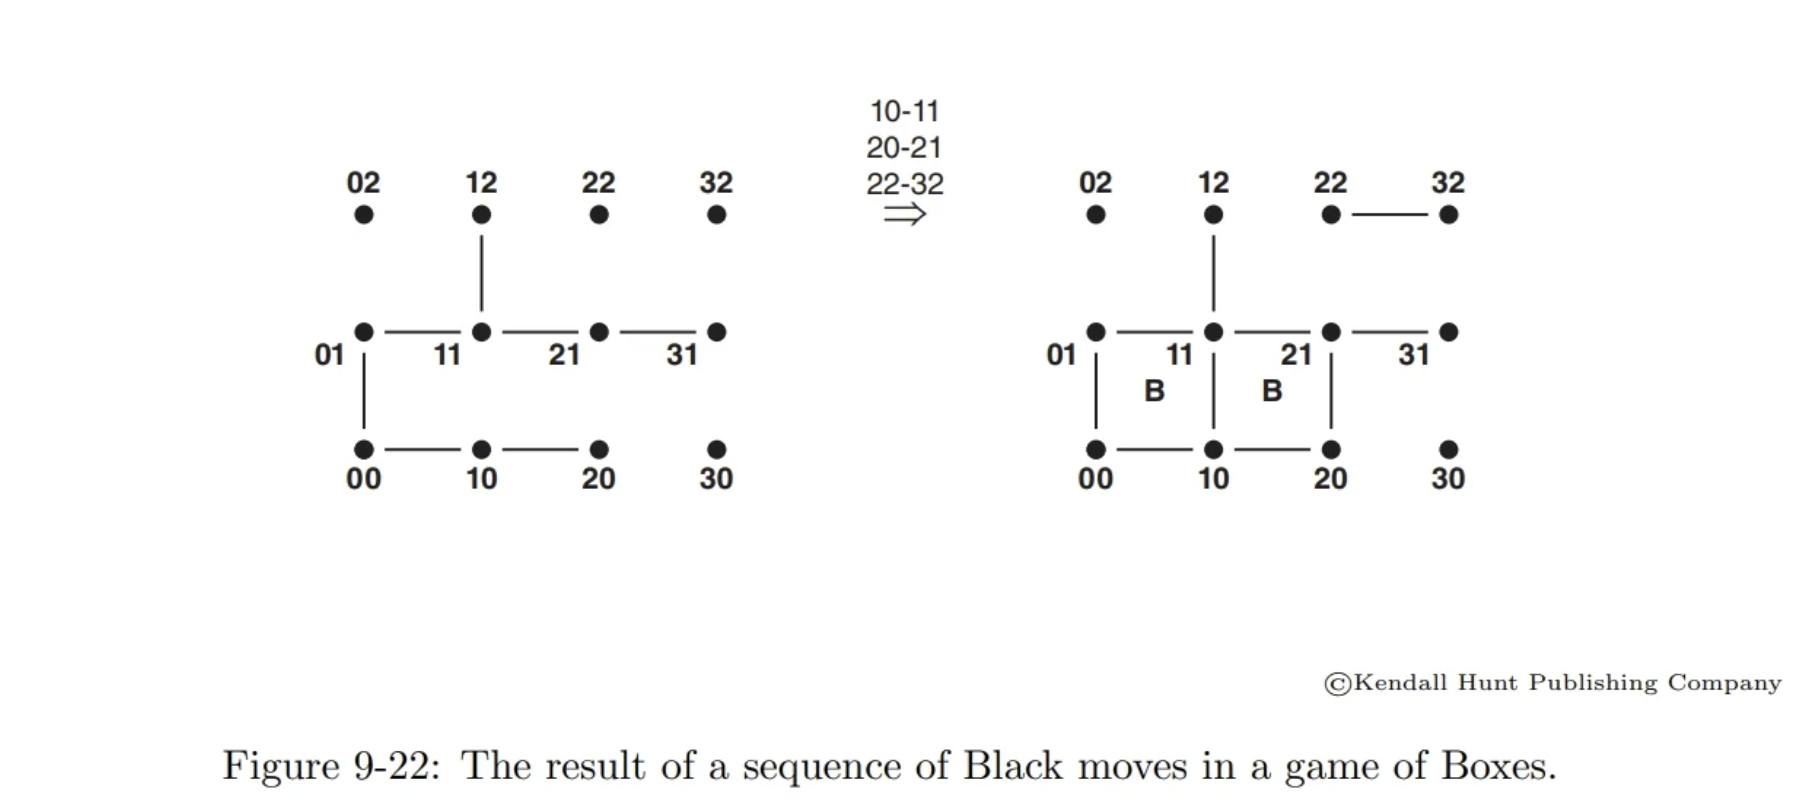
\includegraphics[width=1\linewidth]{9-22.png}
\end{figure}

\begin{enumerate}[(c)]
    \item  The 1 $\times$ 1 game is dull because Black always scores the only point on his second move. Analyze the 1 $\times$ 2 game and determine who wins and by what margin under optimal play. It may help to exploit symmetries – while White has seven possible first moves, you can restrict attention to only three.

\end{enumerate}
\subsection*{\textbf{Solution:}}
\begin{enumerate}[(c)]
    \item 
    because we can assume that both players are playing optimally, they will always tie, the first move optimally will to immediately take the middle because it is a high value spot, and taking that will remove the chance for chaining together squares, they will always avoid making a 3 sided square at all costs so eventually all squares will be 2 sided squares, from there black will be forced to make a 3 sided square and white will gain that point as to not make another 3 sided square, after that they get their bonus move, which they can only use to make a 3 sided square, to which black will take and complete the game in a tie everytime.
\end{enumerate}


\newpage
\section*{\textbf{P5.1.7} [10 pts]}
\begin{enumerate}[(a)]
    \item How many strings, as a function of $n$, are in the language ($a$ + $aa$ + $aaa$)$^n$? Prove your answer by induction on $n$.

    \item  Repeat part (a) for the language ($b$ + $ab$ + $aab$)$^n$.
    
\end{enumerate}


\subsection*{\textbf{Solution:}}
\begin{enumerate}[(a)]
    \item the function to find the total number of strings can be represented as $1+2\times n$ because for each higher number n, only 3 new unique strings are added and the smallest is removed, this is because only the 3 additions onto the longest string a matter because all the rest already exist in the language n-1 and the smallest is removed because it can no longer be represented, 2 of the terms can be made up from the other terms, aa can be made with 2 a, aaa can be made with 3 aaa, so each iteration only adds net 2 unique\newline
    base case: $n=1$ then there are 3 strings because a aa aaa occurs\newline
    plug in to hypothesis to show that yes $3 \times 2 + 1$  is 3, assume hypothesis works for all\newline
    prove n+1 exists, when n exists: $2\times (n+1) + 1 = 2\times n + 2 + 1$ which is true because for each iteration n, there are 2 more unique strings in the language 


    \item the function to find the total number of strings can be represented as $3^n$ this is because each iteration of n multiplies the total by 3, for all of the strings, 3 unique strings are being concatenated ( each string is a unique number of a between 2 b, so each addition is unique), thus there are no repeats to be worried about \newline
    base case: $n=1$ $3^1=3$ this is true because b ab aab occur\newline
    prove n+1 exists, when n exists $3^{n+1} = 3^n\times 3$ therefore true because it shows that n+1 is just 3 times more than n
    
\end{enumerate}

\newpage
\section*{\textbf{P5.1.10} [10 pts]}
 A string has a \textbf{double letter} if it has a substring of the form $aa$ where $a$ is a letter of $\sum$.
\begin{enumerate}[(a)]
    \item Write a regular expression for the set of strings over $\sum$ = $\{a$, $b\}$ that have no double letter. Justify your answer.

    \item We’ll see later that the set $X$ of strings over $\sum$ = $a$, $b$, $c$ that (1) start with $a$, (2) end with $a$, and (3) have no double letter, is denoted by the regular expression $a(ba$ + $c(bc)^*a$)$^*$. For now, explain why every string in this expression’s language meets the three conditions for membership in $X$.
    
\end{enumerate}

\subsection*{\textbf{Solution:}}
\begin{enumerate}[(a)]
    \item to have no double letter repeats, then there must be a b between every aa, and vice verca, therefore if it starts with a, then its some length combo of ab or ba starting with either letter too \newline
    the regex will be a combo of $a,b,(ab)*,(ba)*,a(ba)*,b(ab)*$ so either a or b or ababab or babababa or ababa or bababab\newline
    therefore the full regex will be $(ab)*+(ba)*+a(ba)*+b(ab)*$
    \item because it starts and ends with a, the regex has the a in the beginning and the end, now its concatenated with either only ba, or a c concatenated with any number of bc, followed by the a from before, overall the whole pattern can happen any number of times
    
\end{enumerate}


\newpage
\section*{\textbf{P5.2.6} [10 pts]}
 Write a regular expression for the complement of the language denoted by the expression $(b + ab + aab)^*$.

\subsection*{\textbf{Solution:}}
$(a+aaa(a)*)+(b + ab + aab)^*a$
in that expression there will never be more than 2 a in a row and never just an a without a b and never a string that ends in a and this regex represents that
\newpage
\section*{\textbf{P5.4.6} [10 pts]}
 Is it true that for any regular languages $S$ and $T$, ($S^* \cap T$) = $(S \cap T)^*$? Prove your answer.

\subsection*{\textbf{Solution:}}

this is not true, we can prove it by counter example, $T = {a}$ and $S ={b}$
so $(S*\cap T = a,ba,bbbba$ and such like that, meanwhile $(S \cap T)*=\emptyset ,ab,abab$ and such like that, we can easily see that these are not equivalent
\newpage
\section*{\textbf{P5.5.1} [10 pts]}
 If L is a language and $a$ is a letter, we define the \textbf{quotient of} $L$ \textbf{by} $a$, written $La^{-1}$, as follows. $La^{-1}$ consists of all those strings that $would$ $be$ in $L$ $if$ you appended an $a$ to them --- formally, $La^{-1}$ = $\{w : wa \in L\}$. Prove that if $S$ is any regular expression, and $a$ is any letter, then $L(S)a^{-1}$ is a regular language. Give a recursive algorithm to produce a regular expression for this language.

\subsection*{\textbf{Solution:}}
if we can represent the language as a DFA, then we know that it is a regular language, we know L is regular, we just \newline
$La^{-1}=\{ a,$ anything ending in a $\}$ so minimum length is 1 and number of states is 1+1=2 it can be represented by this figure 
\begin{figure}[h]
    \centering
    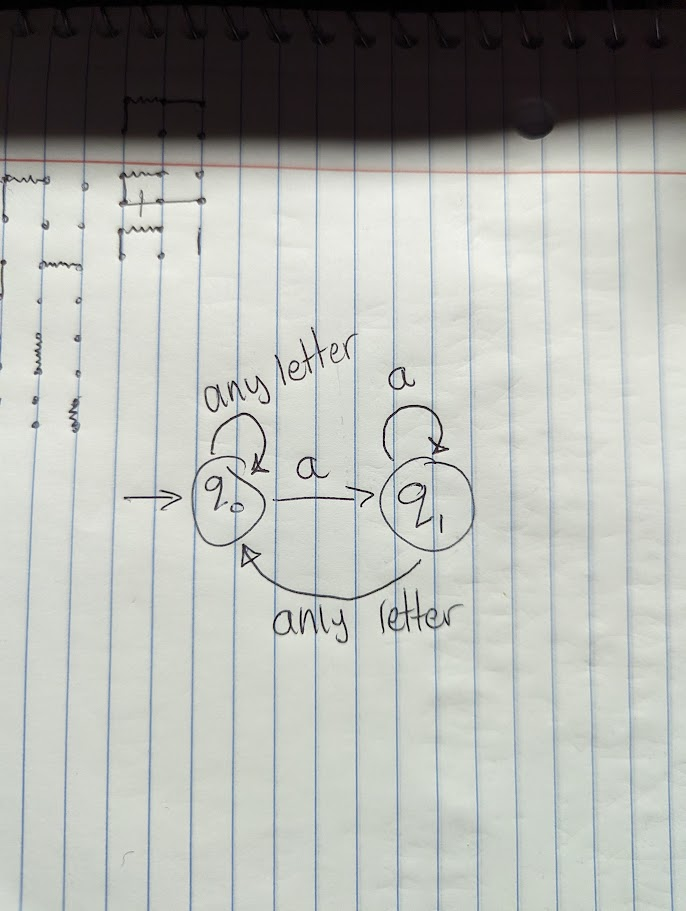
\includegraphics[width=0.25\textwidth]{PXL_20240427_005457934.jpg}
\end{figure}
because adding a character to the end of any DFA just adds 1 more state, and is still valid so it is still a regular language that can be represented by some regular expression\newline
a recursive algorithm could be a representation of the DFA: \newline
\begin{verbatim}
    language(regex, L){
        if regex match L:
        {
            return: add a to the end of regex
        }
        create regex that matches L
        return: language(created regex, L)
    }

\end{verbatim}


\newpage


\section*{\textbf{EC: P9.10.3} [10 pts]}
Analyze the rook-king-king game of Exercise 9.10.3 and determine the winning positions for White and the drawing positions for Black. (The number of valid positions is far smaller than what you calculated there.)

\subsection*{\textbf{Solution:}}
when white have the first move, they will always win as long as they avoid putting their rook into a position to be captured. they will eventually corner black king into the corner and win\newline
for black to force a draw is to have the board in a position such that the black king can capture the white rook without being put into mate, so either the white rook moves to a spot where it can be captured, or black king starts right next to the rook and have it be blacks turn, then once there are 2 kings a stalemate is forced.

\end{document} 